\documentclass{sig-alternate}
\usepackage{verbatim}
\usepackage{graphicx,subfigure,multirow}
\usepackage{epstopdf}
\usepackage{comment}
\usepackage{array}
\usepackage{mathtools}
\usepackage{amsmath}
\usepackage{color}
%\usepackage{times}
\usepackage{multirow}
\usepackage{balance}
\usepackage{url}
\usepackage{eurosym}
\makeatletter
\newif\if@restonecol
\makeatother
\let\algorithm\relax
\let\endalgorithm\relax
\usepackage[vlined, boxed,linesnumbered]{algorithm2e}


\newcommand{\tabincell}[2]{\begin{tabular}{@{}#1@{}}#2\end{tabular}}
\newcommand{\tc}[1]{\multicolumn{1}{c}{#1}}


\newcommand{\reminder}[1]{\textbf{[** #1 **]}}  % to fix
\newcommand{\hide}[1]{} %hide
\newcommand{\vpara}[1]{\vspace{0.05in}\noindent\textbf{#1 }}
\newcommand{\para}[1]{\vspace{0.01in}\noindent\textbf{#1 }}
\newcommand{\secref}[1]{Section~\ref{#1}} %section reference
\newcommand{\Real}{\ensuremath{\mathbb{R}}}  % Real numbers
\newcommand{\figref}[1]{Figure~\ref{#1}} %section reference
\newcommand{\beq}[1]{\begin{equation}#1\end{equation}}
\newcommand{\beqn}[1]{\begin{eqnarray}#1\end{eqnarray}}
\newcommand{\beal}[1]{\begin{align}#1\end{align}}
\newcommand{\besp}[1]{\begin{split}#1\end{split}}
\DeclareMathOperator*{\argmin}{arg\,min}
\DeclareMathOperator*{\argmax}{arg\,max}

% from JH
\newcommand{\from}[2]{{\bf [{\sc from #1:} #2]}}
\newcommand{\eg}{{\sl e.g.}}
\newcommand{\ie}{{\sl i.e.}}
\newcommand{\etc}{{\sl etc.}}
\newcommand{\etal}{{\sl et al.}}
\newcommand{\wrt}{{\sl w.r.t.}}
\newcommand{\omitmark}{{... \sl[Omitted]}}


\hide{
% Package to generate and customize Algorithm as per ACM style
\usepackage[ruled]{algorithm2e}

\renewcommand{\algorithmcfname}{ALGORITHM}
\SetAlFnt{\small}
\SetAlCapFnt{\small}
\SetAlCapNameFnt{\small}
\SetAlCapHSkip{0pt}
\IncMargin{-\parindent}
}

%\newcommand{\eeq}[1]{\end{equation}\normalsize}

\newdef{definition}{Definition}
\newdef{problem}{Problem}
\newdef{theorem}{Theorem}
\newtheorem{hypothesis}{Hypothesis}
\newtheorem{assumption}{Assumption}


\newcommand{\bm}[1]{\textcolor{blue}{#1}}


\begin{document}

\title{
Debiasing Crowdsourced Annotation \\ on Small Batches of Data Items
}

\numberofauthors{1}
\author{
\alignauthor Honglei Zhuang \\
\affaddr{University of Illinois at Urbana-Champaign}  \\
\email{ hzhuang3@illinois.edu}
% \alignauthor Jiawei Han \\
% \affaddr{University of Illinois at Urbana-Champaign}  \\
% \email{ hanj@illinois.edu}
}
%
% Put no more than the first THREE authors in the \author commandpp

% NOTE: All authors should be on the first page. For instructions
% for more than 3 authors, see:
% http://www.acm.org/sigs/pubs/proceed/sigfaq.htm#a18


\maketitle


\begin{abstract}

Crowdsourcing is the de-facto standard for gathering annotated data.
While, in theory,
data annotation tasks are assumed to be attempted by workers independently,
in practice,
data annotation tasks are often grouped into batches to be presented
and annotated by workers together,
in order to save on the time or cost overhead of providing instructions or necessary background.  
Thus, even though independence is usually assumed between annotations on data items within the same batch,
in most cases, a worker's judgment on a data item can still be affected by other data items within the batch, leading to additional errors in collected labels.
%Although annotation bias of individual data items and sequential data items has been explored,
%little research has been done on batches of data items.
%Grouping data items in batches can facilitate crowdsourced data annotation of a great number of tasks
% (\eg~clustering, outlier detection~\etc).
In this paper, we study the data annotation bias when data items are presented as batches
to be judged by workers simultaneously.
We propose a novel worker model to characterize the annotating behavior on data batches,
and present how to train the worker model on annotation data sets.
We also present a debiasing technique to remove the effect of such annotation bias
from adversely affecting the accuracy of labels obtained.
\zhl{
Our experimental results on both synthetic data and real-world data 
demonstrate that our proposed method can achieve up to +57\% improvement in terms of $F_1$-score 
comparing to the majority voting strategy.  
%and up to +14-17\% improvement comparing to a tuned majority voting strategy.  
}
%the effectiveness of our proposed method.

\hide{
Data annotation bias is found in many situations.  Often it can be ignored
as just another component of the noise floor.  However, it is especially
prevalent in crowdsourcing tasks and must be actively managed.  Annotation
bias on single data items
has been studied with regard to data difficulty, annotator bias, etc., while
annotation bias on batches of multiple data items simultaneously presented to
annotators has not been studied.  In this paper, we verify the existence of
``in-batch annotation bias'' between data items
in the same batch.  We propose a factor graph based batch annotation model to
quantitatively capture the in-batch annotation bias, and measure the bias during a
crowdsourcing annotation process of inappropriate comments in LinkedIn.  We
discover that annotators tend to make polarized annotations for the entire batch
of data items in our task.  We further leverage the batch annotation model to propose a
novel batch active learning algorithm.  We test the algorithm on a real
crowdsourcing platform and find that it outperforms in-batch bias na\"{\i}ve
algorithms.
}

\end{abstract}



% A category with only the three required fields
\category{H.2.8}{Database Applications}{Data mining}
%\category{H.3.3}{Information Search and Retrieval}{Text Mining}
\category{J.4}{Social and Behavioral Sciences}{Psychology}
%\category{H.4.m}{Information Systems}{Miscellaneous}
%\terms{Algorithms, Experimentation}

\keywords{Crowdsourcing; annotation bias; worker model}

\sloppy

%!TEX root=betamain.tex


\section{Introduction}
\label{sec:intro}

Crowdsourcing provides an efficient method 
to annotate data on a large scale for various machine learning tasks
by employing a massive workforce drawn from global Internet users.
Popular online crowdsourcing platforms include
Amazon Mechanical Turk\footnote{\url{https://www.mturk.com/}} and CrowdFlower\footnote{\url{http://www.crowdflower.com/}}.
However, while crowdsourcing is relatively cheap compared
to employing experts, getting large quantities of training data
annotated by crowds (say thousands, or millions of data items) 
can be rather expensive. 
% However, in contrast to data annotated by experts,
% crowdsourced annotation usually suffers from a relatively higher level of errors, 
% due to crowd workers' lack of expertise or experience.  
%which limits the adoption of crowdsourcing as a regular method of annotated data collection.

A key mechanism, often employed in practice for reducing costs, is {\em batching},
i.e., grouping multiple data items (to be annotated together) into one single
task as a batch. 
Batching can save significant monetary costs, since the necessary instructions
and background for completing the task needs to be provided just once
for the entire batch. 
Thus, the worker will spend less time on reviewing these instructions, 
and more time on annotating data items, and therefore will be able to
annotate more data items within the same time. 
For instance, consider a scenario where a worker has to judge whether
a comment is relevant to a document. 
Here, making a judgment for each comment requires reading through the entire 
document.
Instead, with batching, the worker only needs to read the entire document
once, and then make a judgment for all the comments in the batch. 
% Typically, in practice, multiple questions or data items are grouped into batches
% to be sent to workers on crowdsourcing platforms.
% First, sending batches of data items can save cost,
% as the necessary instructions or background for completing the tasks needs to be provided only once,
% limiting the overhead when the workers have to read elaborate instructions or necessary background before labeling each data item.
% Consider an example where a worker has to judge whether a comment is relevant to a certain document.  
% Here making a judgment on each comment requires reading through the entire document.
In fact, even from the workers' point of view,
it is also more attractive to label batches of data items
as they can save time on switching between different tasks.
Furthermore, once they start on a batch,
they no longer have to ``fight'' for other high paying or attractive tasks.

%


\begin{figure*}[!t]
  \centering
  %\begin{subfigure}[b]{0.62\columnwidth}
  \subfigure[Data items judged independently]{
    \label{subfig:example_ind}
   % \centering
    \begin{tabular}{@{}cc@{}}
    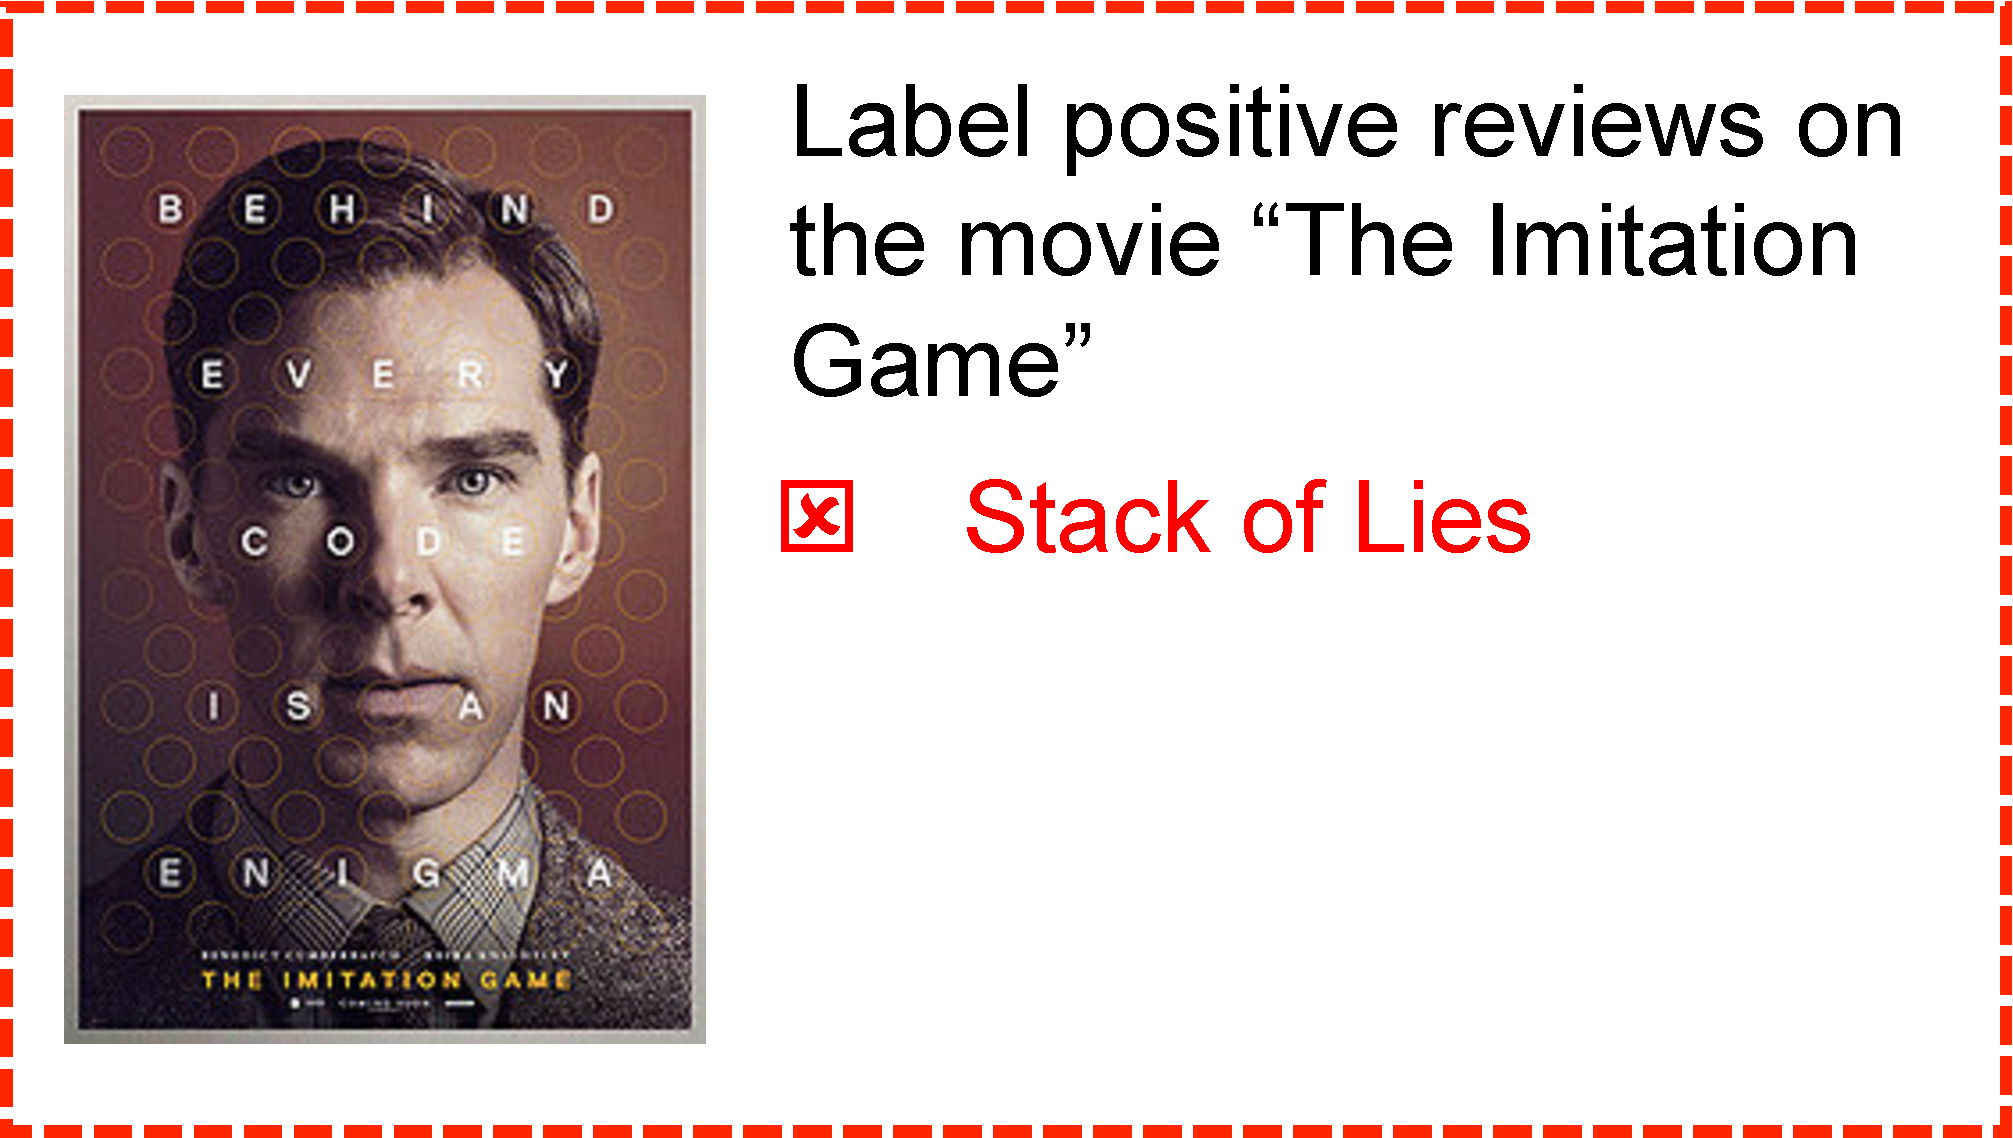
\includegraphics[width=0.30\textwidth]{figures/example_movie_ind1} &
    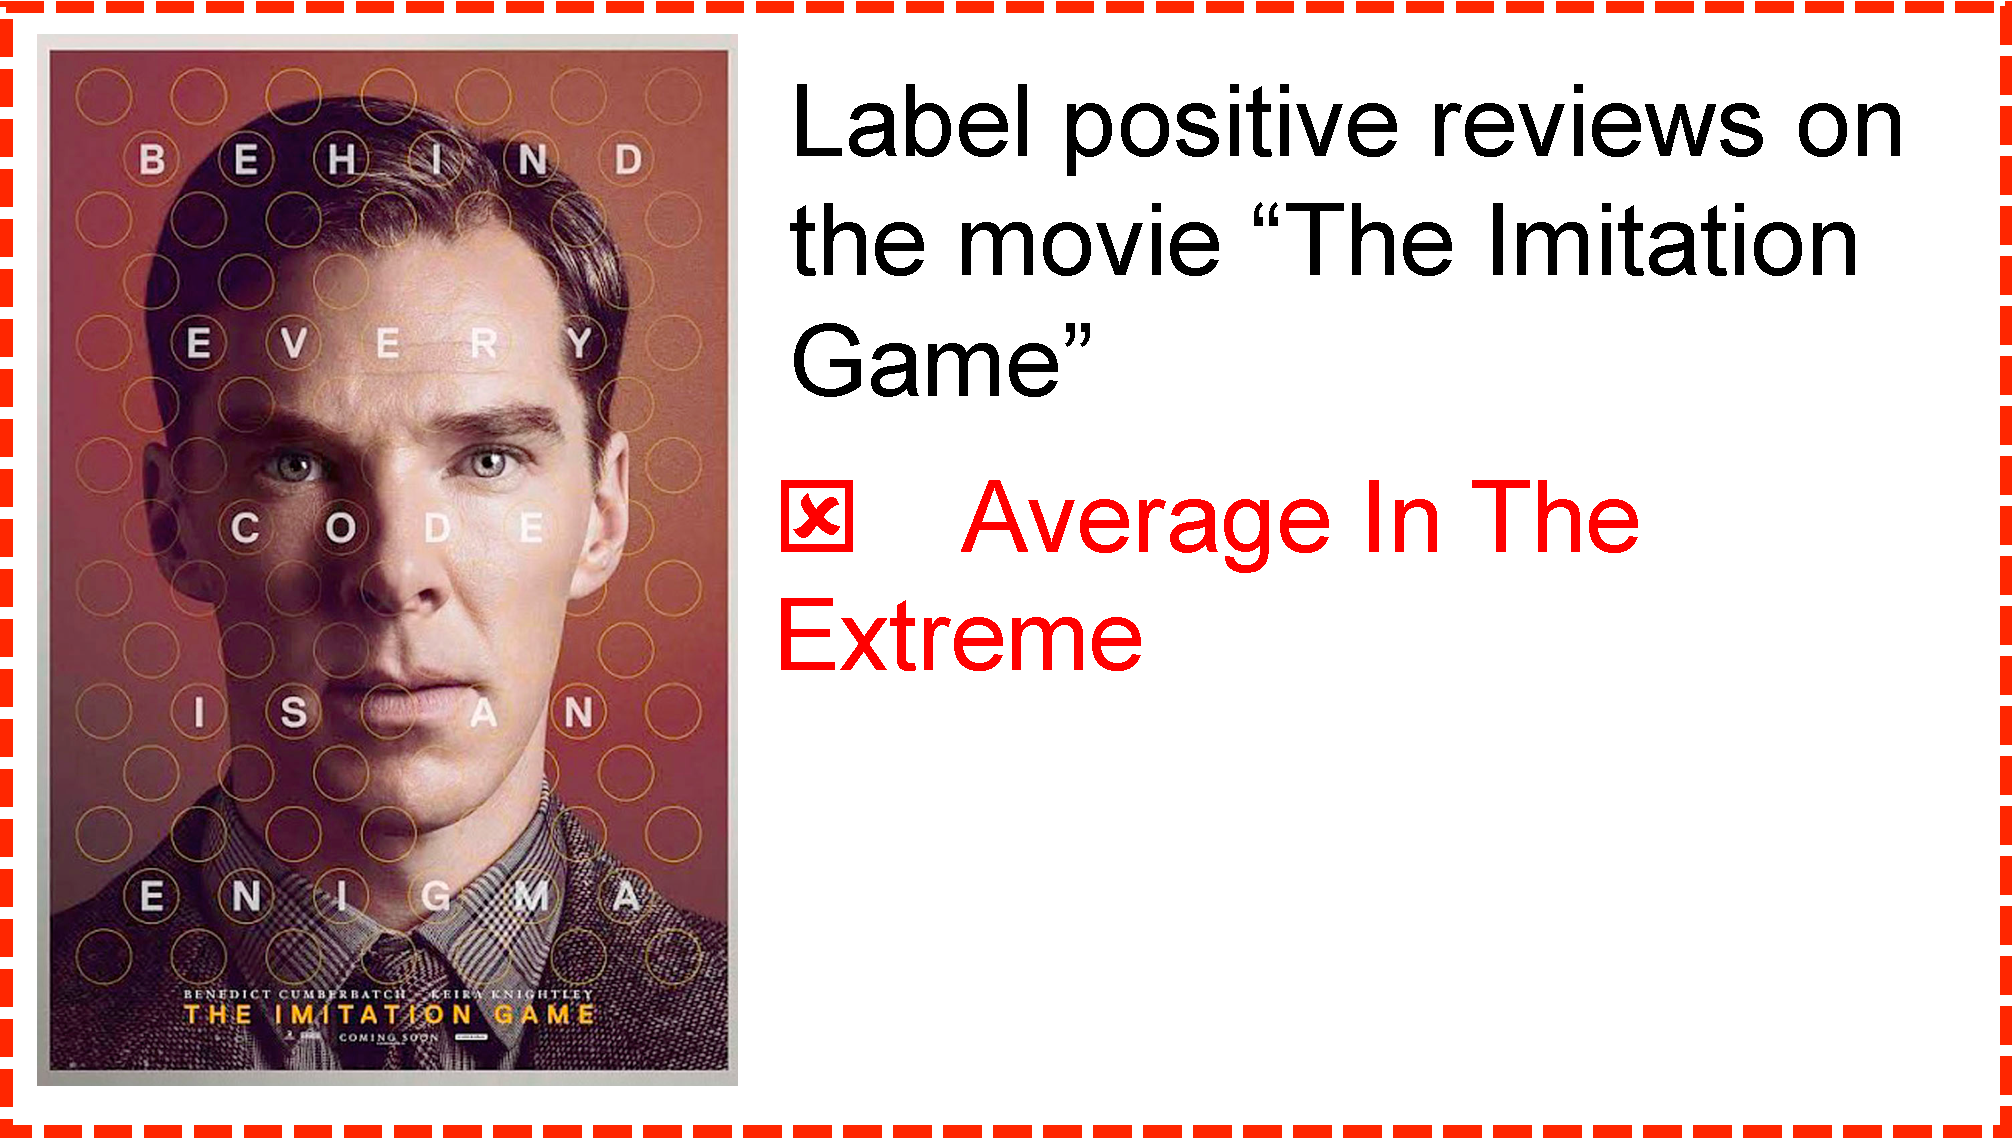
\includegraphics[width=0.30\textwidth]{figures/example_movie_ind2} \\
    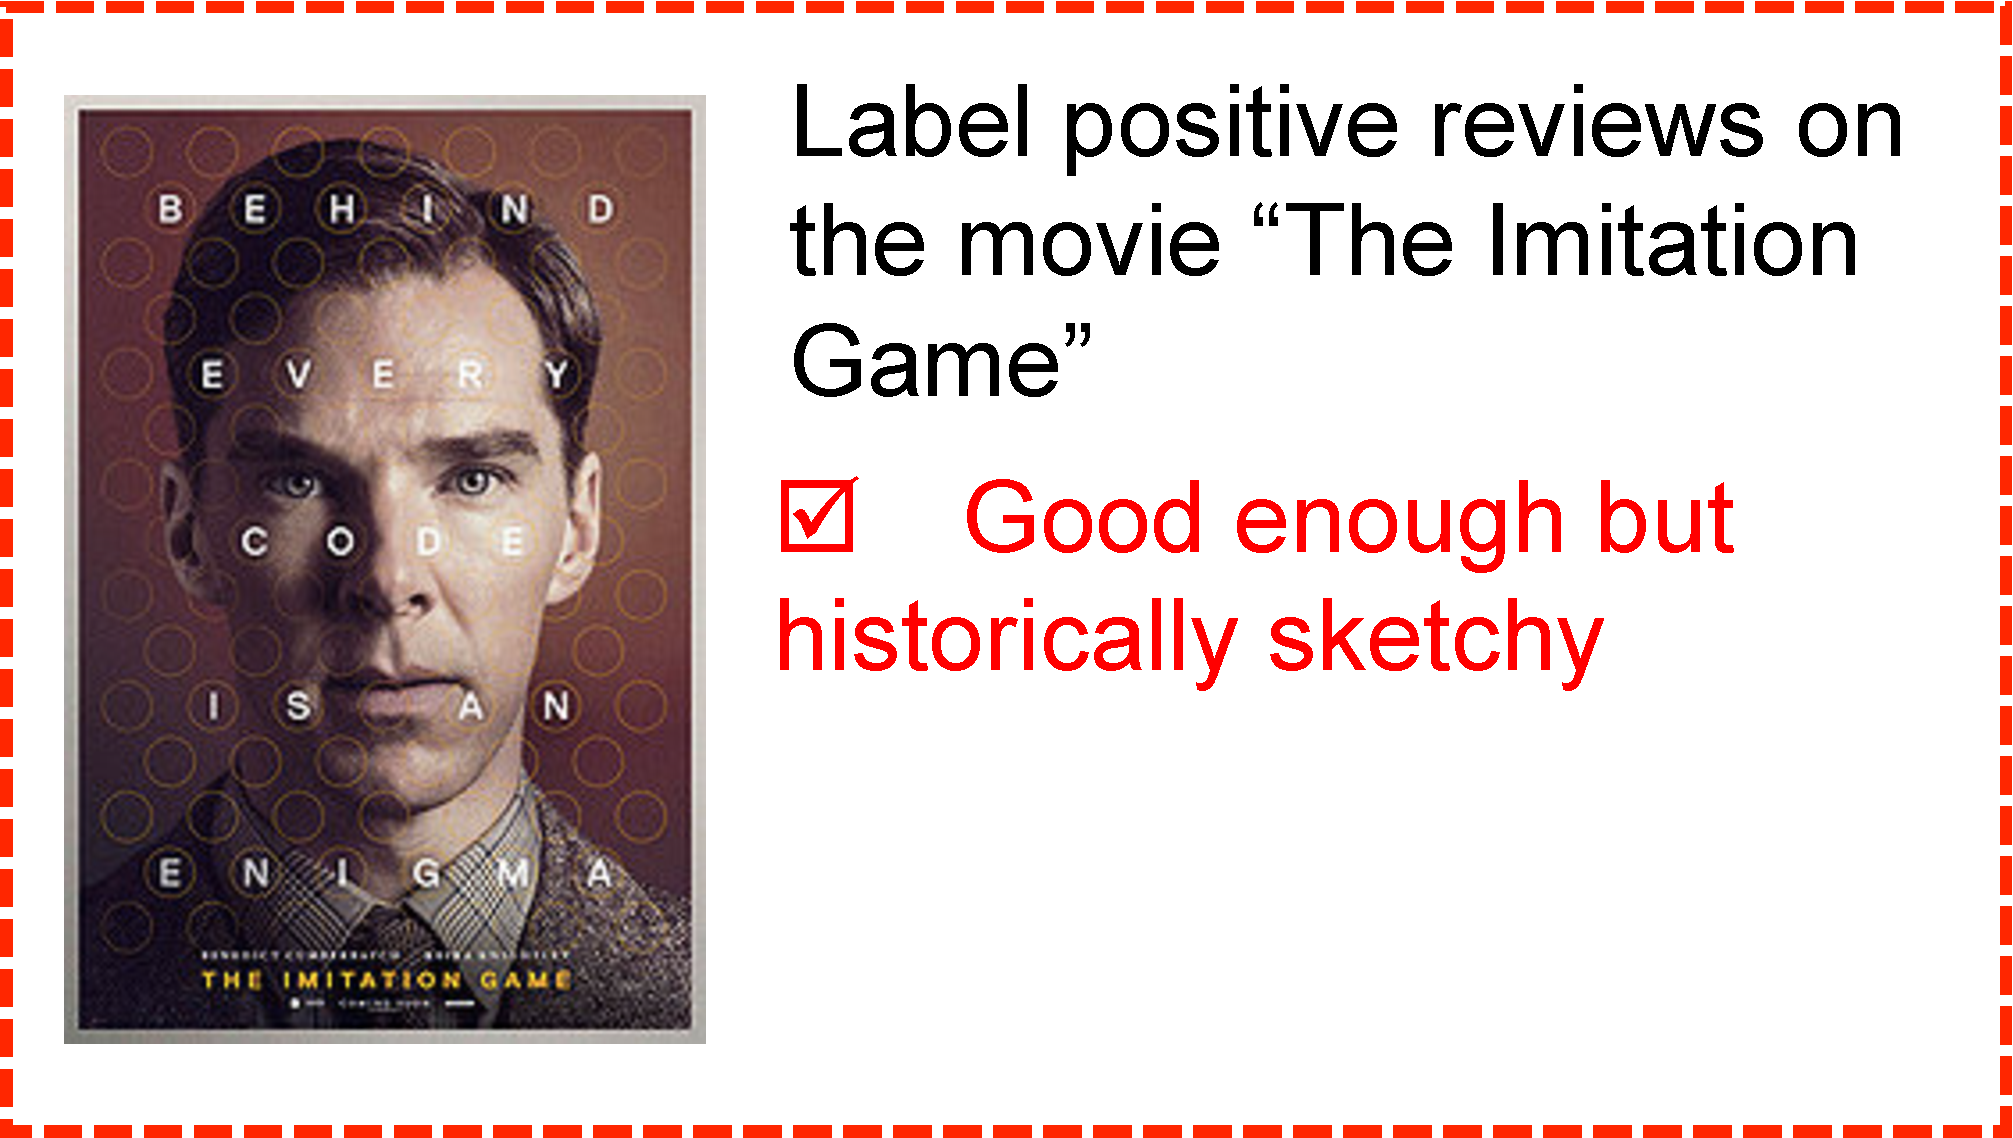
\includegraphics[width=0.30\textwidth]{figures/example_movie_ind3} &
    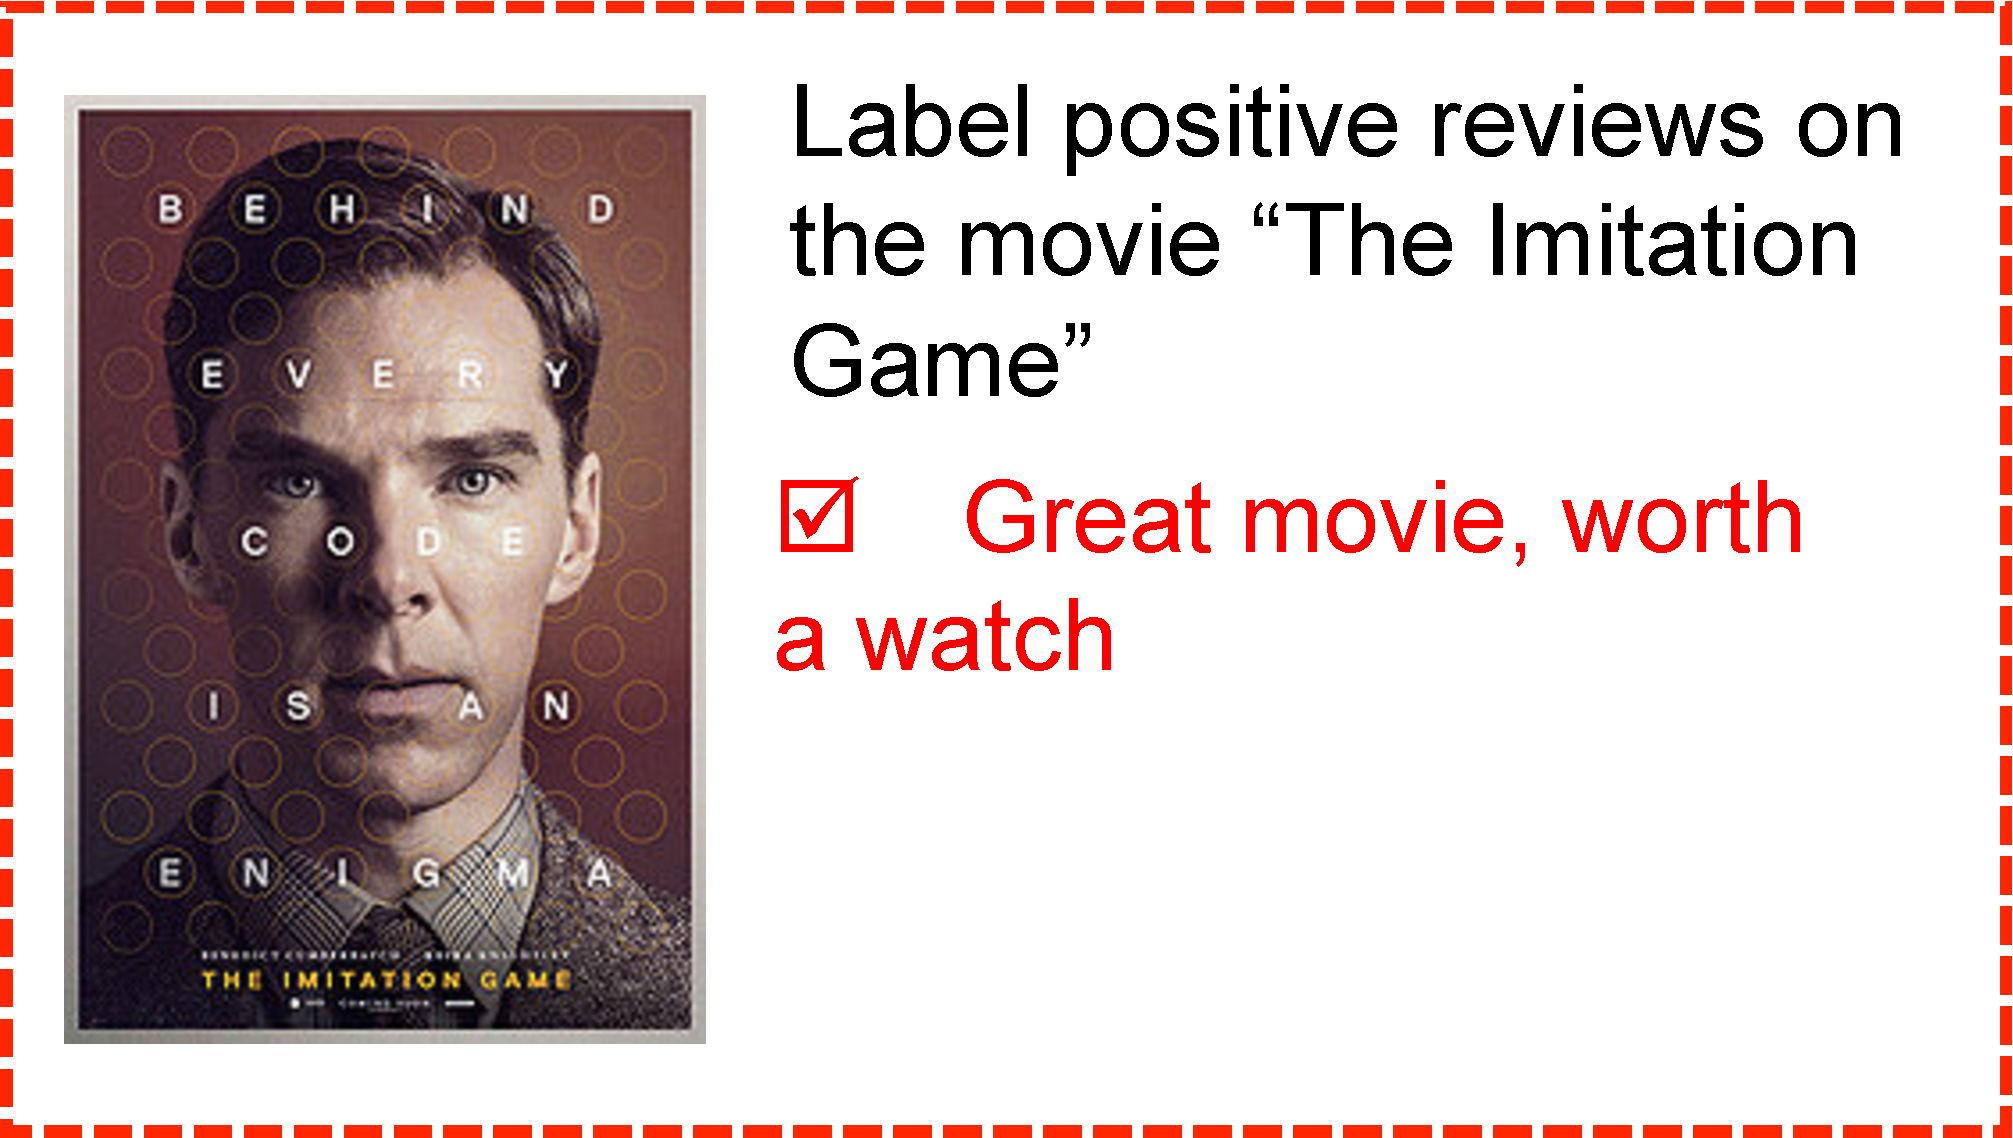
\includegraphics[width=0.30\textwidth]{figures/example_movie_ind4}
    \end{tabular}
  }
   % \caption{Data items judged independently}
  %\end{subfigure}
  %\begin{subfigure}[b][0.31\columnwidth]
  \subfigure[Data items judged in a batch]{
    \label{subfig:example_batch}
    %\centering
    \begin{tabular}{@{}c@{}}
    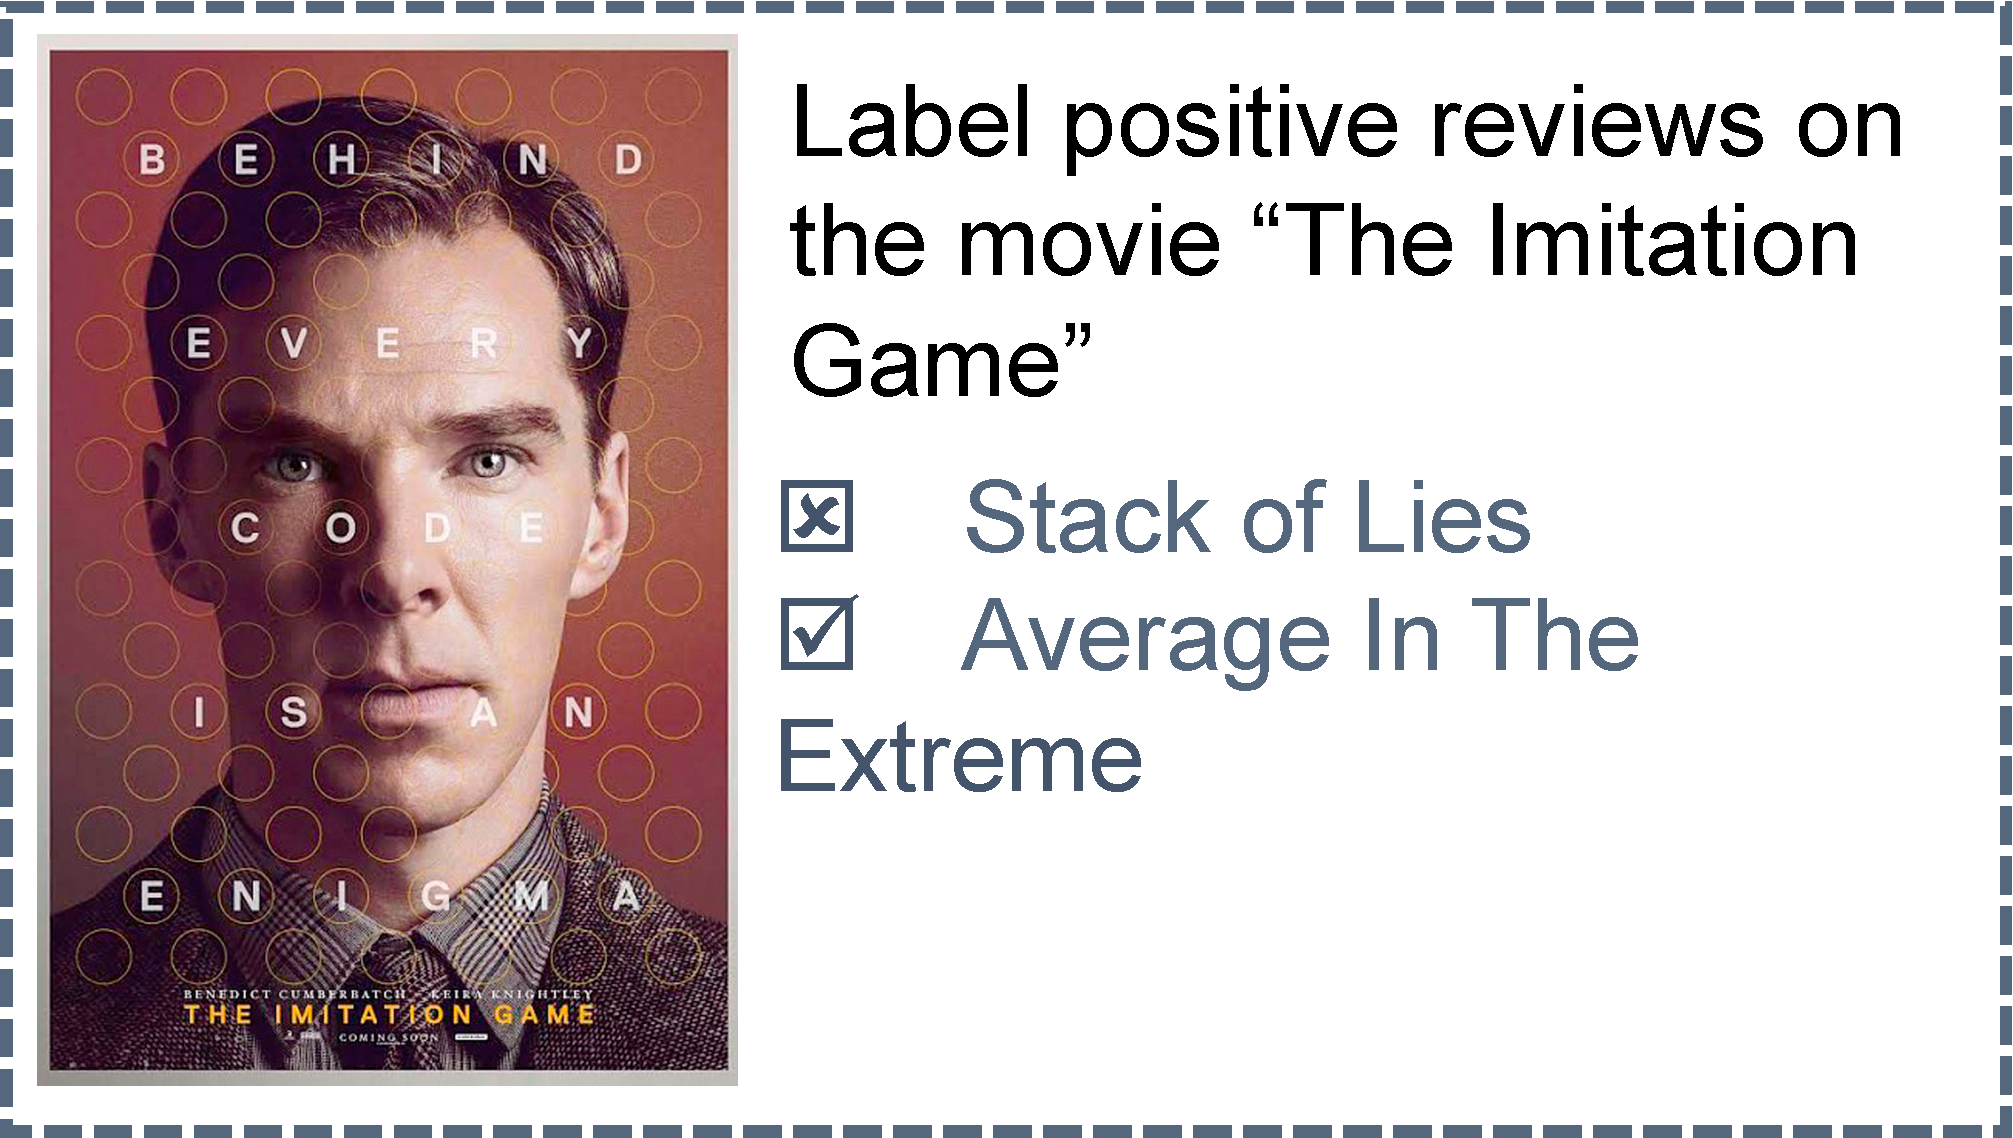
\includegraphics[width=0.30\textwidth]{figures/example_movie_grp1} \\
    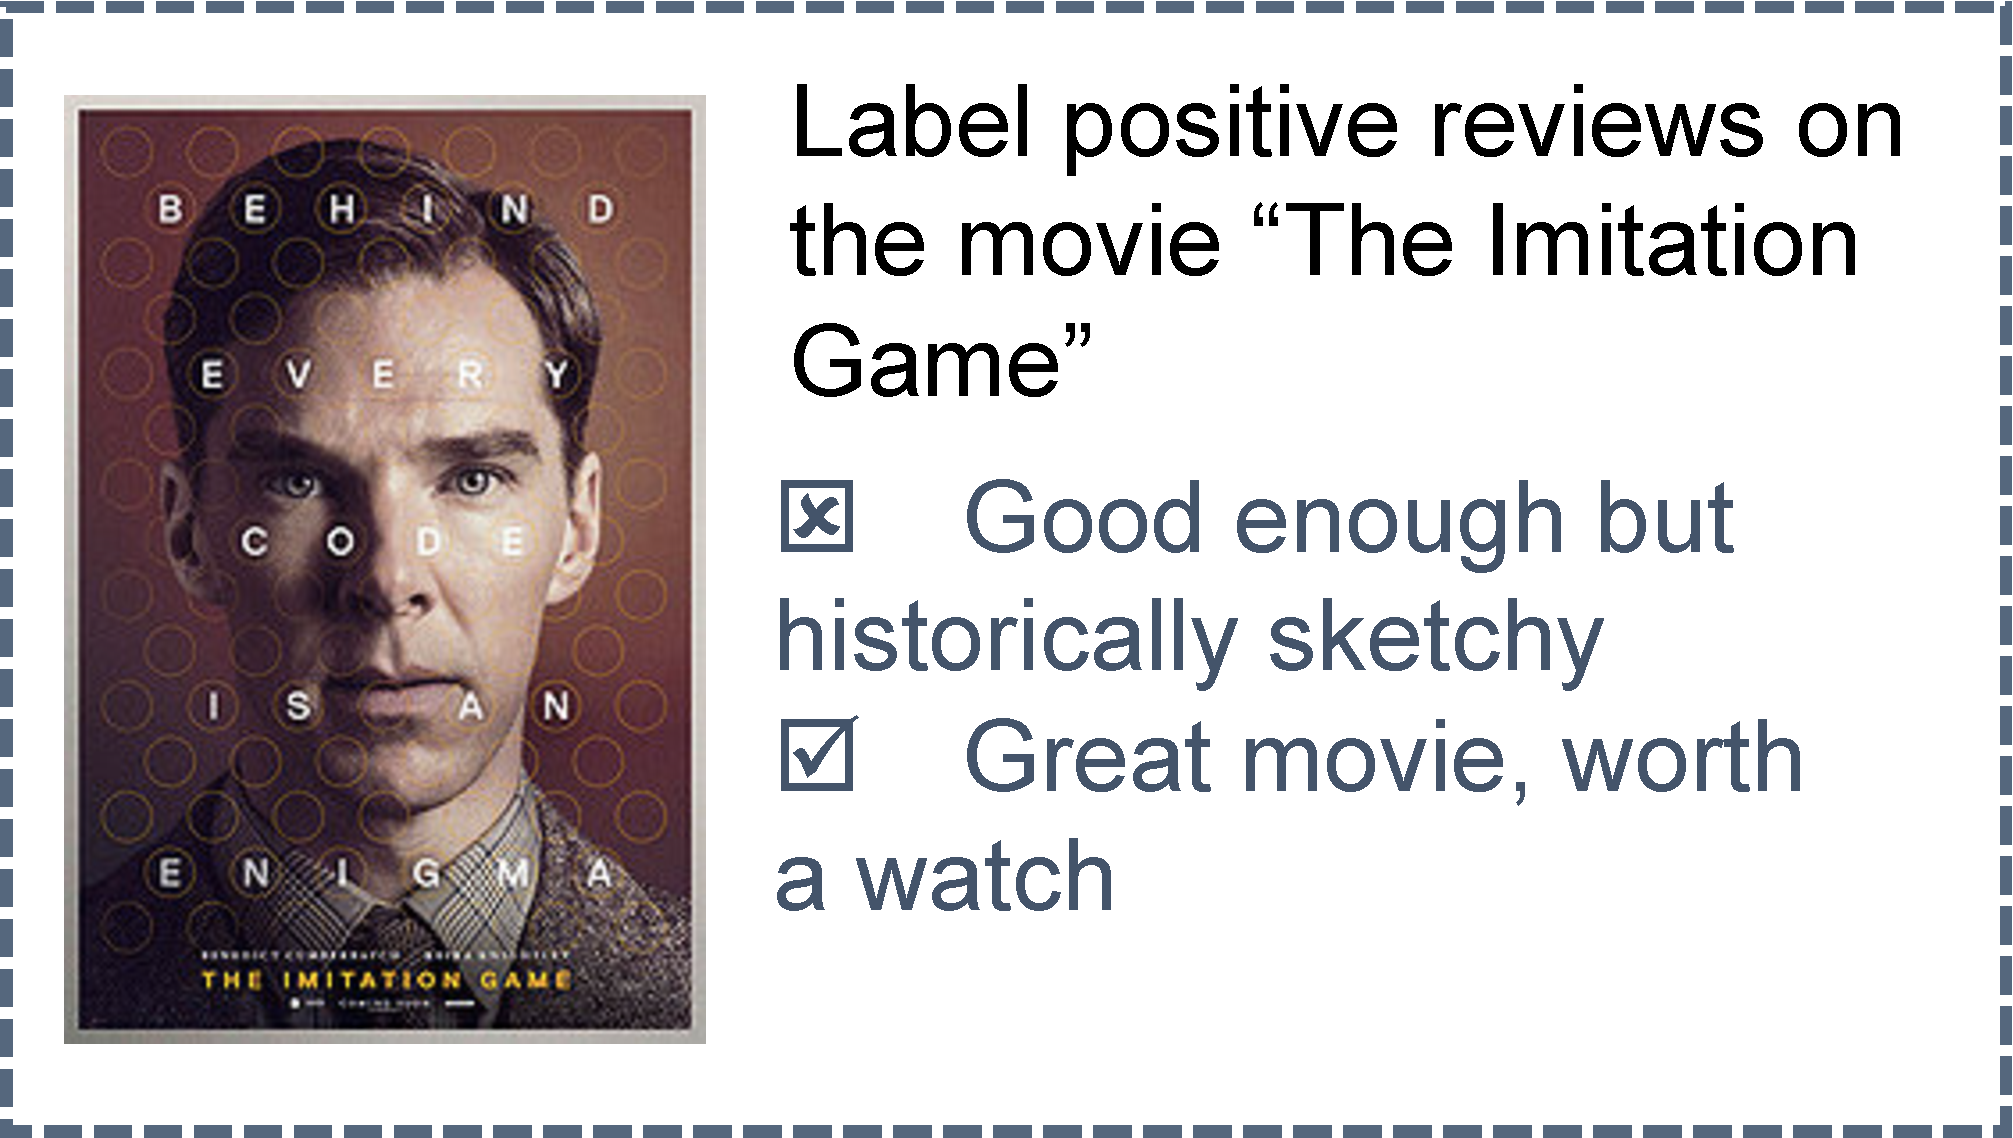
\includegraphics[width=0.30\textwidth]{figures/example_movie_grp2}
    \end{tabular}
  }
    %\caption{Data items judged in a batch}
  %\end{subfigure}
  \caption{\label{fig:example}
  Example of correlation between annotations on data items in the same batch.
  Workers are asked to label whether a review on the movie ``The Imitation Game'' crawled from IMDb is positive.
  Assign each review-movie pair to workers separately can be costly,
  while assigning a batch of reviews together with a movie to workers might affect workers' judgments.
  }
\end{figure*}


\hide{
\begin{figure}[!t]
  \centering
  \subfigure[Data items judged independently]{
    \label{subfig:example_ind}
    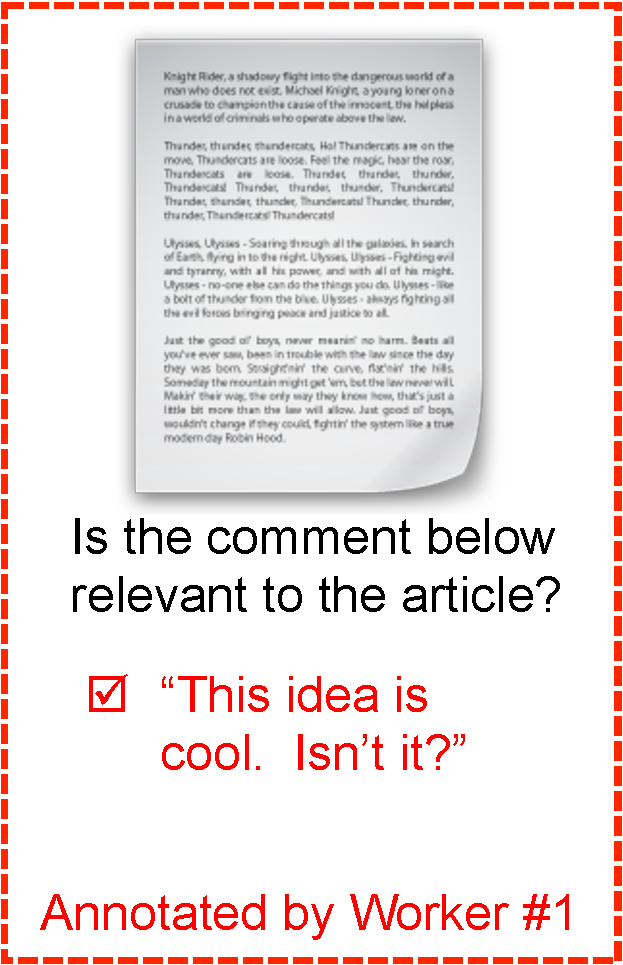
\includegraphics[width=0.30\columnwidth]{figures/example_ind1}
    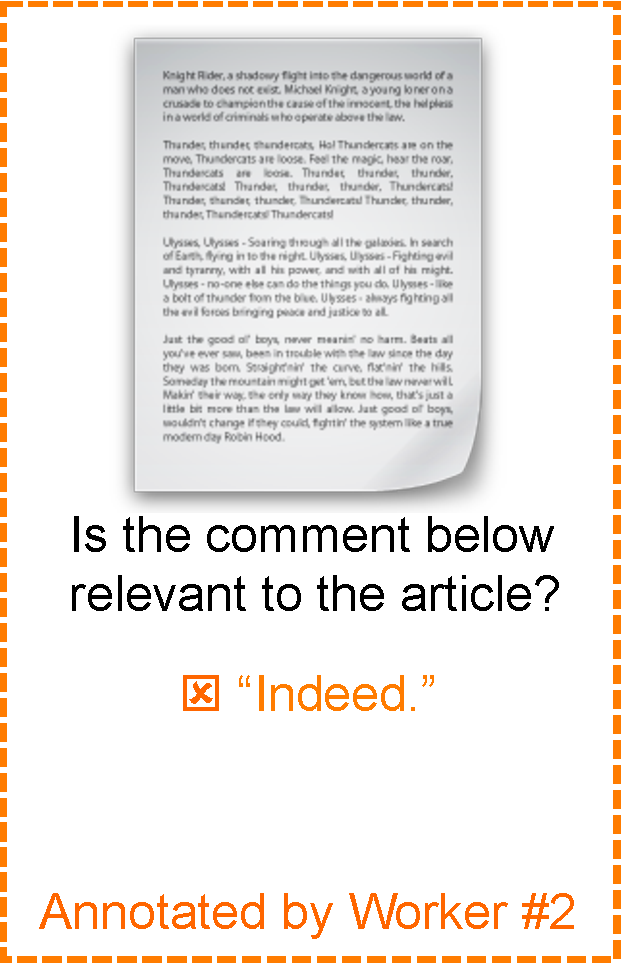
\includegraphics[width=0.30\columnwidth]{figures/example_ind2}
  }
  \subfigure[Data items judged in a batch]{
    \label{subfig:example_batch}
    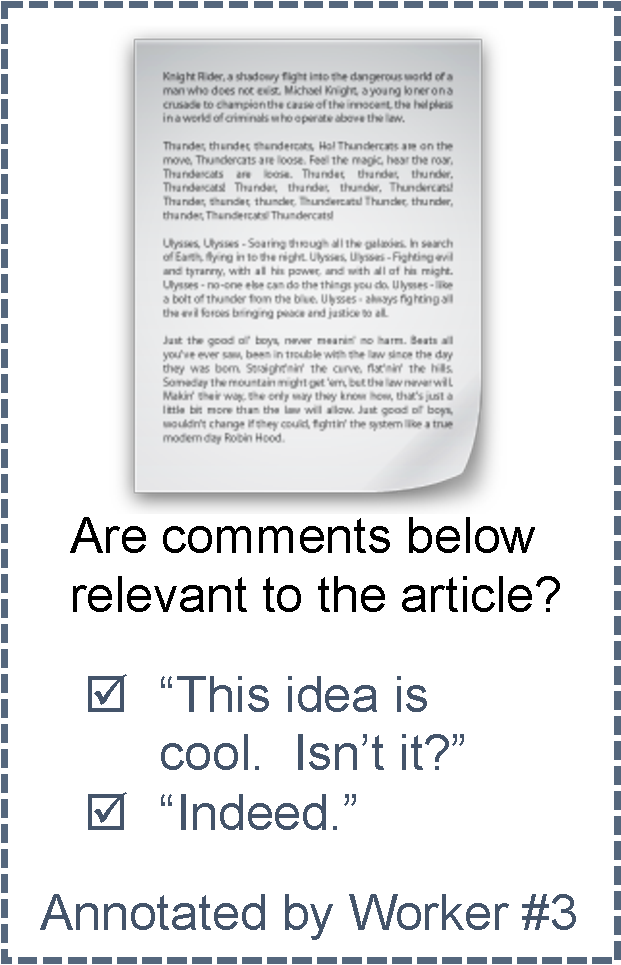
\includegraphics[width=0.30\columnwidth]{figures/example_batch}
  }
  \caption{\label{fig:example}

  }
\end{figure}
}


However, even though batching is an attractive option in practice
due to its cost and time savings, having workers annotate batches can lead to severe correlation between annotations within batches.  
%there could be correlations between annotations made by workers on data items within the same batch.
For example, say we have a task of annotating whether a review of the movie ``The Imitation Game'' crawled from IMDb is positive.
As illustrated in Figure~\ref{subfig:example_ind}, if we only show one review to be judged as part of each crowdsourcing unit task,
workers will have to spend some time reading the instructions
and possibly looking up the movie 
before they can make a single judgment on a review.
Although judgments are likely to be independent, 
this way of assigning work is too costly to be practical.
Instead, if we assemble multiple reviews of the same movie into a batch, as shown in Figure~\ref{subfig:example_batch},
workers can make multiple judgments after they read the instructions.  
Nevertheless, in this case, the annotation of different reviews might interfere with each other.
For example, when the review ``Average In The Extreme'' does not seem like a positive review per se (Cf. top right in Figure~\ref{subfig:example_ind}),
when grouped with the review ``Stack of Lies'', it looks much more like a positive review (Cf. top in Figure~\ref{subfig:example_batch}).
Similarly, when the review ``Good enough but historically sketchy'' looks quite positive by itself (Cf. bottom left in Figure~\ref{subfig:example_ind}),
it does not look as positive as a strongly effusive review simply saying ``Great movie'', as shown in the bottom of Figure~\ref{subfig:example_batch}.
Thus, overall these effects might be undesirable and misleading as it is inconsistent with the case when workers make independent judgments.
Therefore, it is challenging to ascertain true labels of data items in batches.


%p
\hide{
Data annotation bias has been studiend in multiple settings.
Modeling workers' annotating bias on single data items has been studied in a number of studies~\cite{raykar:nips2011ranking,raykar:icml2009,raykar:jmlr2010,whitehill:nips2009}.
In this scenario, data items are presented separately to the workers
and no assumption is made on the interference between judgments on different data items.
We refer to this setting as the \emph{independent judgments}.
Recently, data items annotated in sequence also attracted research attention~\cite{mozer:nips2010,scholer:sigir2013,scholer:sigir2011}.
Observing that a worker usually makes judgments on a sequence of data items,
to some extent there could be dependencies between judgments made on consecutively presented data items.
This setting could be referred to as \emph{sequential judgments}.
}


So far, there has been little to no work in exploring the 
the possible annotation error introduced by grouping 
data items into batches.
Although batching data items has been adopted in many crowdsourced tasks such as
%This judging-in-batch setting has been noticed and adopted in crowdsourcing practices of
sorting~\cite{marcus:vldb2011}, object recognition~\cite{su:aaai2012} or clustering~\cite{gomes:nips2011}, 
and anecdotally very widely used in practice,   
the assumption is often 
that the annotations are collected independently, which is not the case.
While there is limited work on judging data items in sequence~\cite{mozer:nips2010,scholer:sigir2013,scholer:sigir2011},
it is not directly applicable to our setting where a batch of data items are presented and annotated in parallel.
Our previous research~\cite{zhuang:wsdm2015} also noticed this specific type of annotation bias,
but instead of focusing on debiasing,
we exploited the bias to develop an active learning algorithm aiming to improve a certain classifier performance.
We defer the detailed discussion of the related work to Section~\ref{sec:related}.


\hide{
\begin{figure}[!t]
  \centering
  \subfigure[Independent judgments]{
    \label{subfig:mode_ind}
    
\includegraphics[width=0.95\columnwidth]{figures/mode_ind}
  }\\
  \vspace{0.2in}
  \subfigure[Sequential judgments]{
    \label{subfig:mode_seq}
    
\includegraphics[width=0.95\columnwidth]{figures/mode_seq}
  }\\
  \vspace{0.2in}
  \subfigure[Batch judgments]{
    \label{subfig:mode_batch}
    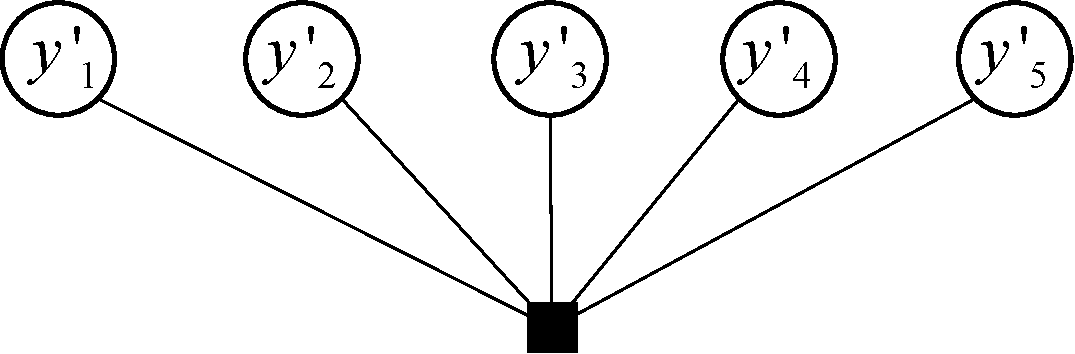
\includegraphics[width=0.95\columnwidth]{figures/mode_batch}
  }
  \caption{\label{fig:worker_mode}
  Graphical model examples of three different scenarios of crowdsourced annotation:
  independent judgments usually occur with interfaces where data items presented separately;
  sequential judgments apply to the case when data items are presented in a long sequence;
  batch judgments usually apply to the scenario when data items are presented in a relatively small batch.
  Circles of $y_i'$ denote random variables representing the annotation given by workers,
  while black boxes are factor functions modeling the dependencies.
  }
\end{figure}
}

There are several research challenges in solving this problem.
First, how do we model workers' behavior when they make judgments in batches?
Second, how do we leverage the model to debias the crowdsourced annotation of data batches?
We make the following contributions in answering these questions:
\begin{enumerate}
  \item \emph{Proposing an interpretable worker annotation model on small batches of data.}
        We propose a novel worker model for binary annotation behavior with data items presented as batches.
        The model incorporates independent judgments and batch judgments based on ranking.
        Different from the factor graph model in our previous work~\cite{zhuang:wsdm2015},
        we focus on obtaining the true labels of data items instead of improving classifier performance.
  \item \emph{Debiasing annotation data obtained as batches.}
        Based on our proposed worker model, we provide an algorithm to debias the inferred labels
        when they are collected from data items in small batches.
  \item \emph{Conducting experiments on a real-world crowdsourcing platform.}
        We conduct experiments on both synthetic and real-world crowdsourcing data sets
        to verify the effectiveness of our proposed model and debiasing strategies.
        Experimental results show the effectiveness of our debiasing method over other baselines.
        %the F1-score of the inferred labels on the real data set can be raised from 88\% to 90\%.
\end{enumerate}

The rest of this paper is organized as follows:
Section~\ref{sec:prelim} introduces the background of crowdsourcing, and formalizes the research problem;
Section~\ref{sec:worker} proposes the worker model for annotating small batches of data;
Section~\ref{sec:debias} presents a strategy to debias batch annotations;
Section~\ref{sec:exp} describes experimental results;
Section~\ref{sec:ext} discusses extensions of our proposed method;
Section~\ref{sec:related} presents related work and Section~\ref{sec:conclusion} concludes.







\section{Preliminaries}
\label{sec:prelim}

We start by introducing the background of a crowdsourcing platform, CrowdFlower.
Then we define the notations used in this paper and formalize the research problem we study.  

\subsection{Crowdsourcing Platform}

We briefly introduce the background of an online crowdsourcing platform, CrowdFlower\footnote{\url{http://www.crowdflower.com/}}.  
On CrowdFlower, users can design and submit a job to the online platform.
The platform will automatically assign the job to global crowd workers (termed as ``contributors'' in CrowdFlower).  
Each ``job'' submitted consists of a data set, an instruction of how the data set should be labeled 
and the interface designed for workers to interact with the platform.
A data set contains several ``units'', and each unit may be assigned to multiple workers to work on.  
Each worker can generate a ``judgment'' for each unit.  
Units are the minimum piece of work to be priced and assigned to workers.  
However, for some tasks the minimum unit price (\ie~0.01 USD) might be too high,
and it would be extremely inefficient for workers to judge only a data item in a unit, 
especially when the judgment needs to be done based on some context that potentially may be shared by different data items.  
For example, in the task of identifying whether a document is relevant to a certain query,
if each unit is designed to be a pair of document and query, 
a worker has to read both the query and the document to make a judgment;
in contrast, if a unit is designed to be a query and a batch of documents, 
the worker can read the query once, and make several judgments on multiple documents within a query.  
Thereby workers can save time, 
and users can lower their cost of data annotation.  


For each job, the user can require all the workers to go through a certain number of ``test questions'' 
before they actually start working on the job.  
Test questions are units of which the correct judgment is already known.
Therefore one can evaluate the accuracy of each worker.
Usually workers with an accuracy lower than 70\% on test questions are not allowed to work on the job.  
We believe that these test questions can be better utilized rather than simply calculating the overall accuracy.  
Richer information about worker behavior might be hidden within the judgments of test questions.  
Users can also insert some units with known answers intermingled with other units while workers work on the job,
to monitor the real time accuracy of each worker.  
Similarly, if the accuracy of a worker drops to lower than 70\%, she will be forbidden from working on the rest of the job.

After the judgments from (multiple) workers toward a unit is obtained, 
one can aggregate these judgments by a majority voting strategy to determine the final annotation of this unit.
However, this strategy may not be the best strategy due to the possible annotation bias when each unit contains multiple data items. 
We can also develop other aggregating strategies to apply on the judgments, 
which better recovers the true labels of data items.  


\subsection{Notation and Problem Definition}

First we need to formalize several concepts.  
Suppose we are given a set of data items $X = \{x_i\}$, where $i=1, \ldots, n$.  
Each data item is associated with a label $y_i \in \mathcal{Y}$,
where in a binary classification case, $\mathcal{Y} = \{0, 1\}$.  
Suppose each $(x_i, y_i)$ is generated from a joint probability distribution $P_{\mathcal{X} \mathcal{Y}}$.  
We define $\eta_i$ to be the conditional probability $P(y_i = 1 | x_i)$.  

In a job submitted to a crowdsourcing platform, 
we can assemble several data items into a batch (``unit'' in CrowdFlower terminology).  
Denote all the batches as a set of batches $B = \{b_j\}$ where $j = 1, \ldots, m$.  
Each batch $b_j$ can be represented by an ordered list of indices of data items in the batch, 
denoted as $(b_{j1}, \ldots, b_{jk})$.  
Thereby the batch $b_j$ consists of data items $(x_{b_{j1}}, \ldots, x_{b_{jk}})$.  
We do allow data items to appear in multiple batches in $B$.  
\hide{
Notice that we are only concerned with the scenario when data items are formed into \emph{small batches}.  
Depending on different format of data items, a small batch can have different scale of size.  
For example, in inappropriate comments identification task, we basically confine $k \leq 5$.   }
Also, for the sake of fully utilize the workforce of crowds, 
we only consider the scenario when all the batches in $B$ have the identical size $k$.  

As we assemble data items into small batch, 
each worker has to judge the entire batch as a single judgment.  
Given a batch $b_j$, the judgment provided by a worker can be represented as $y_j' = (y_{j1}', \ldots, y_{jk}')$, 
where $y_{j t}' \in \mathcal{Y}$ is the annotation of the $t$-th data item in $b_j$, given by the worker.  
Noting that the worker annotation $y_{j t}'$ can be different from the true label $y_{b_{j t}}$.  
We denote all the judgments as $Y'$.  
In real world crowdsourcing platform, a batch can actually be judged by multiple workers.  
We can simply regard them as judgments on multiple identical batches indexed differently, but with the same data items.  


Now we formalize the research problem as below:

\begin{problem} {Debiasing Annotation of Small Batches of Data.}
Given a small training set of data items $X_L$ as well as their true labels $Y_L$.  
Assemble these data items into batches $B_L$ and obtain the corresponding annotation from crowds $Y_L'$.  
Then with a larger set of data items $X_U$ without knowing their true labels, 
again assemble data items in $X_U$ into batches $B_U$, and obtain the corresponding annotation from crowds $Y'_U$.  
The goal is, based on the data and annotation collected from training data set 
and the noisy annotation for $X_U$ returned by the crowds, 
infer the true labels $Y_U$ for data items in $X_U$.  
\end{problem}


In this version of definition, we assume identical worker behavior.  
This assumption is not always true, 
but considering the data sparsity in real world crowdsourcing scenario 
(each worker usually answers only 10 test questions), 
building an accurate enough worker model for each worker is not realistic.  




%!TEX root=betamain.tex

\section{Crowdsourcing Worker Annotation Model on Batches}
%\section{Worker Annotation Model On Small Batch of Data}
\label{sec:worker}

In this section, we first describe our model for workers' annotation behavior 
on a small batch of data items;
then we introduce how to train the model based on a training data set.
%finally we presents the parameters of this model learned from a real world data set.

Our key intuition is the follows:
when a worker judges a batch of data items,
she can either:
1) choose to judge data items independently as if they are presented alone; or
2) to rank all the data items according to their relative inherent values
and annotate the top several items as positive, leaving the rest in the batch as negative.

%

\vpara{Plackett-Luce model.}
Before we delve into our model, we first recap a probability model for generating rankings
based on scores associated with items, 
namely the classical Plackett-Luce model~\cite{luce:2005, plackett:1975} introduced in the 70s.
Without loss of generality, suppose we are given a set of items $x_1, \ldots, x_k$.
Each item $x_i$ is associated with a certain score $s(x_i) > 0$.  %\reminder{example needed here.}
Here the score $s(x_i)$ models the tendency of ranking 
$x_i$ higher in a randomly generated ranking and 
can be viewed as a measure of the inherent ``goodness'' of the item.
A ranking of these items can be represented as a bijection $\pi : \{i\}_{i = 1}^k \mapsto \{x_i\}_{i = 1}^k$,
that maps the $i$-th position in the ranking to the item at this position.
\agp{Doesn't this map $i$ to item at position $i$ in the ranking?}
The corresponding ranking list can be represented as
$\pi(1) \succ \cdots \succ \pi(k)$.
In Plackett-Luce model, the probability of generating a ranking $\pi$ is:
\beal{\label{eq:plmodel}
P(\pi) = \prod_{i = 1}^k \frac{s(x_i)}{\sum_{r = i}^{k} s(x_r)}	
}%
The equation above can be interpreted as the following process:
Initially, we have a pool $A$ of all the data items.
Each time one picks an item $x_i$ from a pool $A$ of data 
items with a probability proportional to its score, namely:
\beal{
P(\text{picking $x_i$ from $A$}) = \frac{s(x_i)}{\sum_{x_r \in A} s(x_r)} \nonumber
}
This item is then removed from the pool $A$ and placed at the next position in the ranking.
Repeat this operation until $A$ becomes empty.
The probability of generating a ranking list according to this process is equivalent to the probability described in the Plackett-Luce model.

%

\vpara{Worker model.}
We now introduce our worker model for annotating small batches of data items.
Again, without loss of generality, suppose we are given a batch $\bx_j$ where $x_{jl} = x_l$,
namely the given data item batch can be denoted as $\bx_j=\{x_1, \ldots, x_k\}$.
 %of $(x_1, \ldots, x_k)$, namely $b_{ji} = i$.pp
Also, recall that for each data item $x_i$, we denote its predictive probability $P(y_i = 1 | x_i)$ as $\eta_i$,
which is not explicitly known. \agp{It's odd to call this a predictive probability. Isn't
this a measure of goodness or inherent value?}
%Although this value is not explicitly known,
%we assume the worker has the ability to estimate this value based on the features of data item.

When a worker starts to work on a certain batch of data items,
they may choose to use one of two strategies:
\begin{itemize}
  \item \emph{Independent judging.}
  If the worker has the ability to obtain an 
  estimate of the absolute value $\eta_i$ for each data item, \agp{Why does the ability of obtaining an estimate matter? confused..}
  we suppose the worker judges each data item $x_i \in \bx_j$ independently
  by drawing the annotation $y_i'=1$ with probability $\eta_i$ and $y_i' = 0$ with probability $(1 - \eta_i)$.
  \item \emph{Relative judging.}
  If the worker can only tell the relative propensity of whether a data item is more likely to be positively labeled than another data item \agp{This is not dependent on the items right -- this is a random coin toss, it seems to indicate that it is dependent on the items..},
  without knowing absolute value of $\eta_i$,
  we suppose the worker chooses to first rank all the data items based on their probability of being positive,
  then annotates the top-$\tau$ items in the ranking as positive, leaving the other items annotated as negative.
  To be precise, the worker generates a ranking $\pi$ for $k$ items in the batch according to the Plackett-Luce model,
  with the scoring function defined as $s(x_i) = \eta_i$.
  Then the worker draws an integer $0 \leq \tau \leq k$ from a certain distribution,
  where $p_\tau$ denotes the probability of drawing the integer $\tau$.
  For data items ranked as top-$\tau$ in the ranking,
  denoted as $x_i \in \{\pi^{-1}(1), \ldots, \pi^{-1}(p)\}$ (could be empty if $p = 0$),
  the worker annotates them as $y_i'=1$,
  while other data items not within the top-$\tau$ of the ranking $\pi$ are annotated as $y_i' = 0$.
\end{itemize}
To combine these two different scenarios,
we suppose the worker is able to judge independently with a certain probability $0 < \lambda < 1$,
while with probability $(1-\lambda)$ the worker can only make relative judgments.

\hide{
the worker chooses to judge each data item $x_i$ independently based on the $\eta_i$ value.
More concretely, the worker generates $y_i' = 1$ with probability $\eta_i$ and $y_i' = 0$ with probability $(1 - \eta_i)$.
With probability $(1 - \lambda)$, the worker chooses to first rank all the data items based on their probability of being positive,
then annotates the top-$\tau$ items in the ranking as positive, leaving the other items annotated as negative.
To be precise, the worker generates a ranking $\pi$ for $k$ items in the batch according to the Plackett-Luce model,
with the scoring function defined as $s(x_i) = \eta_i$.
Then the worker draws an integer $0 \leq \tau \leq k$ from a certain distribution,
where $p_\tau$ denotes the probability of drawing the integer $\tau$.
For data items $x_i \in \{\pi^{-1}(1), \ldots, \pi^{-1}(p)\}$ (could be empty if $p = 0$), the worker annotates them as $y_i'=1$,
while other data items not within the top-$p$ of the ranking $\pi$ are annotated as $y_i' = 0$.
}

The intuition of this model is to capture two behavior pattern of workers.
In the independent judging scenario,
workers can remain independent in judging different data items in the same batch,
\agp{replace next phrase with:
with each data item being judged based on its inherent score $\eta_i$.}
with respect to the property of each data item $x_i$ characterized by $\eta_i$.
%use an absolute standard to judge data items from different batches,p
%and therefore remain consistent performance.
Nevertheless, sometimes workers might judge data items 
within a batch by comparison.
In the relative judging scenario,
workers still have the ability to judge the relative 
relationships between data items in the same batch,
which is captured by the Plackett-Luce model for generating the ranking.
In order to determine the labels of data items,
they have an expectation of label distribution,
which is reflected by the distribution of generating $\tau$,
as it characterizes the probability of having $\tau$ positives within $k$ data items.
\agp{check: (For instance, if workers expect
there to be few positive items, then the probability of $\tau$
being low is high, while if workers expect
the batches to be balanced, then the probability of $\tau$ being close to
$k/2$ is high relative to other values of $\tau$.}
However, this distribution does not necessarily 
reflect the correct label distribution.
When they try to apply their expectation 
of the label distribution on the batch, bias might occur.

We summarize the process of generating annotation for a batch of data items in our proposed model as below:

\begin{enumerate}
  \item \label{step:tosscoin}
        Toss a coin $Z \sim Bernoulli(\lambda)$.  \\
        If $Z=1$, go to Step~\ref{step:ind};
        otherwise go to Step~\ref{step:rnk}.
  \item \label{step:ind}
        For each $x_i$, generate $y_i' \sim Bernoulli(\eta_i)$. \\
        Output the results and exit.
  \item \label{step:rnk}
        Generate a ranking $\pi$ based on Plackett-Luce model for data items $x_i$ in the batch.
  \item \label{step:draw}
        Draw $\tau \sim Mult(p_{\tau})$.
  \item \label{step:annotate}
        For the top-$\tau$ items in ranking $\pi$, generate $y_i' = 1$; \\
        otherwise generate $y_i' = 0$.  \\
        Output the results and exit.
\end{enumerate}



\vpara{Model learning.}
The parameters that need to be determined in this worker model include:
the probability of making independent judgments $\lambda$,
and the distribution of the number of positive annotation when making relative judgments,
represented by $p_0, \ldots, p_k$, where $0 \leq p_{\tau} \leq 1$ and $\sum p_{\tau} = 1$.
We assume these two parameters are fixed,
independent of the data items in question.
\agp{check:(Or at least, we assume that the two parameters are fixed
for each new application of our techniques ---
for instance, these parameters for content moderation
may be very different from the same parameters for
spam identification or sentiment analysis).}
%p

Suppose we are given a set of $n_L$ items $X_L$ with their predictive distribution \agp{wasn't this inherent value? just checked -- it's not} $\eta_i$ known. %true labels $Y_L$ known.p
Then, we form them into $m_L$ batches $B_L$, send them to the crowds,
and obtain their annotation from workers, denoted as $Y_L'$.


For simplicity, we write $x_{b_{jt}}$ as $x_{jt}$, and similar to $y_{jt}$ and $\eta_{jt}$.
For each batch $b_j \in B_L$, we denote the set of items annotated by workers as positive as $X_{j}^1 = \{x_{jt} | y_{jt}' = 1\}$,
and the set of items annotated as negative as $X_{j}^0 = \{x_{jt} | y_{jt}' = 0\}$.


We train the model by maximum likelihood estimation.
The likelihood of the obtained annotation can be written as:
\beal{
	L = %\overbrace{\prod_{j=1}^{m_L}}^{\text{across all batches}} \biggl[p
        \prod_{j=1}^{m_L} \biggl[
		\lambda \underbrace{
            \prod_{t=1}^{k} \eta_{jt}^{y_{jt}} (1 - \eta_{jt})^{(1 - y_{jt})}
        }_{\text{independent judging}}
		%\prod_{x_{jt1} \in X_{j}^1} \eta_{jt1} \prod_{x_{jt0} \in X_{j}^0} (1 - \eta_{jt0}) \nonumber \\
		+ (1 - \lambda) \underbrace{
            p_{\tau_j} P(X_{j}^1 \succ X_{j}^0)
        }_{\text{relative judging}}
	\biggr]
}%
where $\tau_j = |X_{j}^1|$ is the number of positive annotation in batch $b_j$;
$P(X_{j}^1 \succ X_{j}^0)$ denotes the probability of generating any rankings $\pi$
that rank items in $X_{j}^1$ higher than any items in $X_{j}^0$,
namely:
\beal{
	P(X_{j}^1 \succ X_{j}^0) = \sum_{\pi \in R(X_{j}^1, X_{j}^0)} P(\pi) \nonumber
}%
where $R(X_1, X_0) = \{ \pi |\pi^{-1}(x_{0}) > \pi^{-1}(x_{1}),  \forall x_{1} \in X_1, x_0 \in X_0 \}$;
and $P(\pi)$ is defined by the Plackett-Luce model, as presented in~\eqref{eq:plmodel}.

Applying an EM-algorithm, where at E-step, we can have
\beal{ \label{eq:e_step}
	\hat{\lambda}_j = \frac{\hat{\lambda} \prod_{t=1}^{k} \eta_{jt}^{y_{jt}} (1 - \eta_{jt})^{(1 - y_{jt})}}
	{\hat{\lambda} \prod_{t=1}^{k} \eta_{jt}^{y_{jt}} (1 - \eta_{jt})^{(1 - y_{jt})} +
	(1 - \hat{\lambda}) \hat{p}_{\tau_j} P(X_{j}^1 \succ X_{j}^0)}
}

And at M-step, we update the parameters $\hat{\lambda}$ and $\hat{p}_{\tau}$ by
\beal{ \label{eq:m_step}
	\hat{\lambda} = \frac{1}{m_L}\sum_{j=1}^{m_L} \hat{\lambda}_j, \hspace{0.2in}
	\hat{p}_{\tau} = \frac{1}{\hat{Z}} \sum_{j=1}^{m_L} (1 - \hat{\lambda}_j) \mathbf{1}_{\{ |X_{j}^1| = \tau\}}
}%
where $\hat{Z} = \sum_{j=1}^{m_L} (1 - \hat{\lambda}_j)$.


However, in real data sets, we do not always know $\eta_i$ for each data item $x_i$,
but only know their binary true labels $Y_L$.
We can still learn the worker model based on this situation
by substituting their labels $y_i \in \{0, 1\}$ into $\eta_i$.
Directly substituting the value of 0 or 1 into $\eta_i$ may cause numerical problems in calculating $\lambda_j$.
Therefore we regularize the score by using:
\beal{
	\eta_i = \frac{y_i + \epsilon}{1 + 2 \epsilon} \nonumber
}%
where $\epsilon$ is a small constant which is set to $10^{-3}$ in our experiments.






\section{Debiasing Annotation}
\label{sec:debias}

In this section, we introduce given the trained worker model, 
how to debias annotation collected for small batches of data.  
More precisely, given a set of $n_U$ unlabeled data items $X_U$,
assemble them into $m_U$ batches represented by $B_U$,  
as well as their annotation obtained from the crowds $Y_U'$,
how to infer their true labels $Y_U$.  

The basic idea is, based on the given worker model,
try to infer $\eta_i$ for each $x_i \in X_U$,
then we simply apply the Bayes classifier to determine the inferred label, 
which yields $\hat{y}_i = 1$ if $\eta_i > 0.5$, or $\hat{y}_i = 0$ if $\eta_i \leq 0.5$.  

We again adopt a maximum likelihood estimate.  
The log-likelihood of the obtained annotation is:
\beal{
	\log L (\eta) = \sum_{j=1}^{m_U} 
	\log \biggl[ 
		&\hat{\lambda} %\prod_{t=1}^{k} \eta_{jt}^{y_{jt}} (1 - \eta_{jt})^{(1 - y_{jt})} 
		\prod_{x_{jt1} \in X_{j}^1} \eta_{jt1} \prod_{x_{jt0} \in X_{j}^0} (1 - \eta_{jt0}) \nonumber \\
		+ &(1 - \hat{\lambda}) \hat{p}_{\tau_j} P(X_{j}^1 \succ X_{j}^0)  
	\biggr] 
}%

Notice that $\hat{\lambda}$ and $\hat{p}_{\tau_j}$ are parameters learned from Section~\ref{sec:worker},
and $P(X_{j}^1 \succ X_{j}^0)$ is also a function of $\eta_{i}$'s.  
Similarly, we apply an EM-algorithm here 
by first calculating $\hat{\lambda}_j$ for each batch at E-step basically according to~\eqref{eq:e_step} 
but replacing $\lambda$ and $p_{\tau}$ by the value we learned during the training step.  
Then we can have
\beal{\label{eq:em_debiasing}
	\log L(\eta) &\geq \sum_{j=1}^{m_U} 
		\hat{\lambda}_j \biggl[ 
			\sum_{x_{jt1} \in X_{j}^1} \log \eta_{jt1}  + \sum_{x_{jt0} \in X_{j}^0} \log (1 - \eta_{jt0}) 
		\biggr] \nonumber \\
		& + \sum_{j=1}^{m_U} (1 - \hat{\lambda}_j) \bigl[\log \hat{p}_{\tau_j}  + \log P(X_{j}^1 \succ X_{j}^0) \bigr] 
}%
where the second term includes $\log P(X_{j}^1 \succ X_{j}^0)$, which is hard to optimize.  
We apply the idea of EM-algorithm again here.  
We use notation $R_j$ to represent $R(X_{j}^1, X_{j}^0)$.  
For each $\pi \in R_j$, we can calculate its conditional probability given $X_{j}^1 \succ X_{j}^0$, denoted as $\hat{q}_{\pi}$ by:
\beal{
	\hat{q}_{\pi} = P(\pi | X_{j}^1 \succ X_{j}^0; \hat{\eta}) = \frac{P(\pi; \hat{\eta})}{\sum_{\pi \in R_j}P(\pi; \hat{\eta})} 
}%
which is the E-step.  
According to Jensen's inequality we have:
\beal{\label{eq:semi_ranking_to_sum_of_ranking}
	\log P(X_1 \succ X_0) &= %\log \sum_{\substack{\pi: \forall x_{1} \in X_1, x_0 \in X_0, \\ \pi^{-1}(x_{0}) > \pi^{-1}(x_{1}) }} P(\pi)
	\log \sum_{\pi \in R_j} P(\pi) \nonumber \\
	&\geq \sum_{\pi \in R_j} \hat{q}_{\pi} \log P(\pi)
}%
where the last inequality yields the objective function we want to optimize.  
The correctness of EM-algorithm guarantees the convergence of optimizing this function.  


\hide{
We further utilzie Jensen's inequality to bound this term from bottom by
\beal{\label{eq:semi_ranking_to_sum_of_ranking}
	\log P(X_1 \succ X_0) &= %\log \sum_{\substack{\pi: \forall x_{1} \in X_1, x_0 \in X_0, \\ \pi^{-1}(x_{0}) > \pi^{-1}(x_{1}) }} P(\pi)
	\log \sum_{\pi \in R_j} P(\pi) \nonumber \\
	&\geq \frac{1}{|R_j|} \sum_{\pi \in R_j}  \log P(\pi)
}%
where 
}


Furthermore, according to the minorization-maximizaion algorithm used in~\cite{hunter:aos2004}, 
we can obtain the lower bound for $\log P(\pi)$, which is defined by the Plackett-Luce model, by:
\beal{\label{eq:mm_algorithm}
	\log P(\pi) &= \sum_{t=1}^{k-1} \biggl[ 
		\log \eta_{\pi^{-1}(t)} - \log \sum_{s=t}^{k} \eta_{\pi^{-1}(s)}
	\biggr] \nonumber \\
	&\geq \sum_{t=1}^{k-1} \biggl[ 
		\log \eta_{\pi^{-1}(t)} - \frac{\sum_{s=t}^{k} \eta_{\pi^{-1}(s)}}{\sum_{s=t}^{k} \hat{\eta}_{\pi^{-1}(s)}}
	\biggr]
}%
where $\hat{\eta}_i$ is the estimated parameter of last iteration.  



By combining \eqref{eq:em_debiasing},~\eqref{eq:semi_ranking_to_sum_of_ranking} and \eqref{eq:mm_algorithm}, 
we can obtain the objective function to optimize as:
\beal{\label{eq:objective_function}
	Q(\eta) &= \sum_{j=1}^{m_U} 
		\hat{\lambda}_j \biggl[ 
			\sum_{x_{jt1} \in X_{j}^1} \log \eta_{jt1}  + \sum_{x_{jt0} \in X_{j}^0} \log (1 - \eta_{jt0}) 
		\biggr] \nonumber \\
		&+ \sum_{j=1}^{m_U} (1 - \hat{\lambda}_j)  \sum_{\pi \in R_j}  \hat{q}_{\pi}
		\sum_{t=1}^{k-1} \biggl[ 
			\log \eta_{\pi^{-1}(t)} - \frac{\sum_{s=t}^{k} \eta_{\pi^{-1}(s)}}{\sum_{s=t}^{k} \hat{\eta}_{\pi^{-1}(s)}}
		\biggr]  
}%
Notice that $Q(\eta)$ is actually a lowerbound of the original log-likelihood function.  
Moreover, for two EM-step and one MM-step we apply in deriving $Q$-function, 
it is provent that by improving $Q(\eta)$ from this iteration $Q(\hat{\eta})$, 
we can achieve no less improvement on the loglikelihood.  
Therefore optimizing $Q(\eta)$ can also optimizes the loglikelihood.  



Take the derivative, we can obtain
\beal{\label{eq:derivative_of_objective_function}
    \frac{\partial Q(\eta)}{\partial \eta_i} &= 
        \sum_{j \in M_1(i)}\frac{1}{\eta_i}
        + \sum_{j' \in M_0(i)} \frac{ \hat{\lambda}_{j'}}{1 - \eta_i} \nonumber \\
        %&+ \sum_{j \in M_1(i)} \frac{1 - \hat{\lambda}_j}{\eta_i}
        &+ \sum_{j=1}^{m_U} (1 - \hat{\lambda}_j) \sum_{\pi \in R_j} \hat{q}_{\pi} \biggl[
            \sum_{t=1}^{|X_j^1|} \frac{\mathbf{1}_{\{\pi^{-1}(i) \geq t \}}}{
                \sum_{s=t}^{k} \hat{\eta}_{\pi^{-1}(s)}
            }
        \biggr]
}%
where $M_1(i)$ and $M_0(i)$ are defined as $M_y(i) = \{j:x_i \in X_j^y\}$ for $y \in \{0, 1\}$.  
The updating rule can be obtained by solving $\partial Q(\eta) / \partial \eta_i = 0$.  

By iteratively updating the scores to optimize the likelihood of the annotation on test data, 
we can obtain the inferred predictive distribution of each item.  
Based on which, we can determine the inferred binary label for each data item by assigning $y_i'=1$ if $\hat{\eta}_i > 0.5$, 
or $y_i'=0$ otherwise.  
Notice that we do not further tune the threshold in this step, 
as the scores we learned here are expected to be a reasonable estimate of the true $\eta_i$'s. 
Therefore, if the predictive distribution are known, 
learning theory guarantees that by using Bayes classifier (namely to take 0.5 as threshold) 
is supposed to yield the best expected performance.  




\incmargin{1em}
\begin{algorithm}[!t]
       \caption{Debiasing crowdsourced annotation on batches of data items.}\label{alg:debias}
\small
       \KwIn{Data batches $B_U = \{b_j\}$, crowdsourced annotation $Y_U'=\{y_j'\}$; 
             training data batches $B_L$, crowdsourced annotation $Y_L'$, true labels $Y_L$.} 
       \KwOut{Inferred labels $Y_U$.}

       \BlankLine
       \tcp{Training work model;}
       $\hat{\lambda}_j \leftarrow 0.5$; 
       Initialize $\hat{p}_{\tau}$ by random values; \\
       \Repeat{$L$ converged}
       {
           Update $\hat{\lambda}_j$ bfor $\forall 1 \leq j \leq m_L$ y~\eqref{eq:e_step}; \\
           Update $\hat{\lambda}$ and $\hat{p}_{\tau}$ by~\eqref{eq:m_step}
       }

       \tcp{Calculate debiased labels;} 
       \Repeat{$Q(\eta)$ converged}
       {
           Update $\eta_i$ for $\forall 1 \leq i \leq n_U$ by~\eqref{eq:derivative_of_objective_function}
       }
       $y_i \leftarrow \mathbf{1}_{\{eta_i > 0.5\}}$ for $\forall 1 \leq i \leq n_U$; \\
       Output $Y_U$.
\end{algorithm}
\normalsize
\decmargin{1em}



\section{Experimental Results}
\label{sec:exp}

In this section, we conduct experiments on a synthetic data set and a real data set 
to verify the effectiveness of our proposed worker model and debiasing technique.  

\vpara{Data sets.}
We first introdue the data sets we used in this experiments.  



%!TEX root=betamain.tex


\section{Related Work}
\label{sec:related}

%\agp{Say something about the three categories that you list below.}

In this section, we first introduce existing studies on annotation bias of crowds, 
when data items are presented either independently, or in a sequence or batches; 
we then introduce rank aggregation techniques and their application on crowdsourced ranking or rating.  

%\agp{I fixed all the past tense references below. If I missed something, you should fix.}

% \agp{In some cases, it is not sufficient to say that the papers are not on the same topic,
% we need to argue that the techniques are different or the models are different. Take another pass on this section to make sure we say {\em something} about every set of papers.}

\vpara{Annotation bias in independent judgments.}
A number of studies have been conducted on verifying and quantifying annotation bias of crowd workers.  
%However, these studies mainly consider the scenario when data items are judged independently.  
Snow~\etal~\cite{snow:emnlp2008} explore the performance of annotations by non-expert workers for several NLP tasks.
Demeester~\etal~\cite{demeester:wsdm2014} discuss the disagreement between different users on assessment of web search results.

There are also extensive studies on modeling worker behaviors.  
Raykar~\etal~\cite{raykar:nips2011ranking,raykar:icml2009,raykar:jmlr2010}
study how to learn a model with noisy labeling. 
Specifically, they employ a logistic regression classifier, 
and insert hidden variables indicating whether a worker tells the truth. 
%They utilize an EM algorithm to infer the real ground-truth while training the model.
Karger~\etal~\cite{karger:nips2011} propose an iterative algorithm to infer workers' reliability 
and aggregating their answers.  
Whitehill~\etal~\cite{whitehill:nips2009} model the annotator ability, data item difficulty, and infer the true label from the crowds in a unified model.
Most of these work also proposes various generative model to capture worker behavior.  
However, they assume judgments on different data items are independent, 
which is not necessarily true when data items are grouped into batches.  

Venanzi~\etal~\cite{venanzi:www2014} propose a community-based label aggregation model to identify different types of workers, 
and correct their labels correspondingly.  
Das~\etal~\cite{das:kdd2013} address the interactions of opinions between people connected by networks.
They focus on another aspect of dependencies, 
which is the dependencies between workers, 
while in our studies, we are more concerned about dependencies between data items and their judgments.  

% \agp{Say something like: Like this work, many of these papers
% also consider EM-based techniques; however, to the best of our knowledge,
% we are the first to articulate and provide solutions for the problem
% of debiasing of batches -- either at the start or the end of this portion.}


\vpara{Annotation bias in sequential and batch judgments.}
A few researchers also notice the correlation between judgments on different data items, 
but their work are mainly developed in the setting when data items are reviewed in a sequence.  
Scholer~\etal~\cite{scholer:sigir2013,scholer:sigir2011} study the annotation disagreements in 
a relevance assessment data set.  
%TREC data set, which is on relevance assessment tasks in information retrieval.  
They discover correlations between annotations of similar data items.  %, and the estimated time between the two annotation.  
They also explore ``threshold priming'' in annotation, 
where the annotators tend to make similar judgments or apply similar standard on consecutive data items they review. 
%tend to make similar judgments to consecutive data items.  
However, their work focuses on the scenario when data items are organized in a long sequence.  
It confines the dependencies to exist only between consecutive data items.  
Also, they focus more on qualitative conclusions, without a quantitative model to characterize and measure the discovered factors.  
Carterette~\etal~\cite{carterette:effect2010} provide several assessor models for the TREC data set.  
Mozer~\etal~\cite{mozer:nips2010} study the similar ``relativity of
judgments'' phenomenon on sequential tasks instead of batches.  
Again, their focus is more on data items presented as a long sequence, 
while we focus more on data items presented in batches simultaneously.  

Our recent work~\cite{zhuang:wsdm2015} also considers a similar setting 
when data items are organized in batches; 
we verify the existence of annotation bias caused by batching data items.  
Our focus in that paper was to design an active learning algorithm to smartly assemble batches, 
aiming to improve the performance of the classifier trained on this annotation batches.  
Our focus was not on improving the quality of labels collected, 
and we still used majority voting to obtain labels for data items.  
In this paper, we focus on debiasing the obtained labels, 
which can trigger a broader range of application 
including both training and evaluating classifiers.
\hide{
the higher label quality can benefit tasks including training and/or evaluating classifiers, 
with a broader range of applications.
}


\vpara{Crowdsourced ranking and rating.}
In our model, we employ the Plackett-Luce model to capture worker behavior, 
and aggregate worker annotations on batches as rankings in order to infer true labels.  
There is a related thread of work on rank aggregation; 
however, to the best of our knowledge, 
we are the first to model crowds' annotating behavior on batches by ranking, 
and propose a debiasing strategy. 

Studies on aggregating multiple rankings into a consistent ranking can be dated back to the seminal work of Arrow~\cite{arrow2012social}.  
Negahban~\etal~\cite{negahban:nips2012} study how to aggregate pairwise comparisons into a ranking 
by utilizing the Bradley-Terry model~\cite{bradley:1952}, which is a simplified version of Plackett-Luce model utilized in this paper.   
Hunter~\etal~\cite{hunter:aos2004} propose the minorization-maximization (MM) algorithm to infer Plackett-Luce model 
from multiple partial orderings.  
Soufiani~\etal~\cite{soufiani:nips2013} generalize Negahban~\etal's work 
and proposed a class of generalized method-of-moments (GMM) algorithm 
to infer parameters of Plackett-Luce model from multiple orderings, 
and compare the performance against MM-algorithm.  
They then further extend their algorithm 
to be applied to a more general class of ranking models called random utility models (RUMs)~\cite{soufiani:icml2014}.  
In addition, the technique for rank aggregation has also been studied 
in context of information retrieval~\cite{dwork:www2001,klementiev:icml2008,liu:www2007,qin:nips2010,volkovs:www2012}.  
%A summary of early work can be found in~\cite{dwork:www2001}.
These studies do not explicitly address the crowdsourcing settings 
to actually model the worker behavior.  
Directly applying their techniques (\eg~\cite{hunter:aos2004}) may not lead to better performance, 
as shown in our experiments.  

There is related research on aggregating multiple rankings or leveraging crowds' power to obtain ranking of data items.  
Chen~\etal~\cite{chen:wsdm2013} study aggregating crowdsourced annotation on pairwise comparison to obtain a ranking on data items. 
Mao~\etal~\cite{mao:aaai2013} show how aggregated results of noisy voting obtained from crowdsourcing platform 
may differ by using different aggregating strategies.  
However, their objective is just to obtain a ranking, 
while our model incorporates a ranking model but the ultimate goal is still to collect labels for data items.  

%They employed the simplified version of Plackett-Luce model for pairwise comparison, Bradley-Terry model~\cite{bradley:1952}, 
%and extended the model to adapt the crowdsourcing settings.  
%Similar problem is also studied by Volkovs~\etal~\cite{volkovs:www2012}, 
%while they proposed a multinomial preference model for partial ranking of data items.  

%and apply the model on aggregating crowdsourced comparison on data item pairs into a ranking.  
%Furthermore, our model can deal with not only pairwise comparisons, 
%but also the situation with more than two data items in a batch.  

Several papers also consider crowdsourced rating.  
Parameswaran~\etal~\cite{parameswaran:vldb2014} focused on crowdsourced rating on items, 
and applied their system on a peer evaluation data set of a MOOC course.  
Crowdsourcing has also been utilized for rating multimedia content quality~\cite{chen:mm2009} and relevance assessment~\cite{alonso:2008}.  
However, they do not explicitly study the scenario when data items are grouped into batches.  

\hide{
\vpara{Batch active learning.}
Active learning has been extensively studied.
Settles~\etal~\cite{settles:2010survey} summarized a number of active learning strategies.
Batch active learning, in contrast to traditional active learning settings, aims to choose a set of data items to query, which proposes some unique challenges.
Some strategies focus on optimizing the helpfulness of a data batch.
Hoi~\etal~\cite{hoi:icml2006,hoi:www2006} utilized Fisher information matrix to choose the data items that are likely to change the classifier parameters most.
Brinker~\etal~\cite{brinker:icml2003} studied batch active learning for SVM and aimed to maximize the diversity within the selected set of data samples.
Guo~\etal~\cite{guo:nips2008} proposed discriminative active learning strategy by formulating the problem as an optimization problem.
% Azimi~\etal~\cite{azimi:icml2012} propose a Monte-Carlo method to sequentially select the batch of samples to query.
A number of strategies also aim at choosing the most representative data batch with regard to the unlabeled data set.
Yu~\etal~\cite{yu:icml2006} proposed a transductive experimental design, which prioritizes the data samples that represent the hard-to-predict data.
Chattopadhyay et al.~\cite{chattopadhyay:kdd2012} tried to choose the data batch to minimize Maximum Mean Discrepancy (MMD) to measure the difference in distribution between the labeled and unlabeled data.
There are studies addressing both intuitions.
Wang~\etal~\cite{wang:kdd2013} designed a framework to minimize the upper bound of empirical risk, which aims to find a batch of data items that are both discriminative and representative.
However, all of the above studies assume reliable oracles---which never are in multiple-annotator scenarios such as crowdsourcing.

\vpara{Active learning with crowds.}
Crowdsourcing serves as a potentially ideal oracle for active learning.
Two perspectives have been explored; 
first is how to select data items to query when the oracles are noisy.
Sheng~\etal~\cite{sheng:kdd2008} provided an empirical study on the performance of repeated labeling and developed an active learning strategy addressing both the ``label uncertainty'' and ``model uncertainty''.
Second is how to select annotators for crowdsourcing.
Donmez~\etal~\cite{donmez:kdd2009} studied this problem, by modeling the querying problem as a multi-armed bandit problem.  Each annotator is regarded as as a bandit, and a binary reward function is defined based on whether the oracle provides a correct label.  %However, the true label is unknown. They hence utilize majority voting to determine the ground truth.
Yan~\etal~\cite{yan:icml2011} explore both the problem of selecting query samples and selecting oracles, in context of a logistic regression classifier.
Kajino~\etal~\cite{kajino:aaai2012} proposed a convex optimization function for active learning in crowds.  
% vijayanarasimhan~\etal~\cite{vijayanarasimhan:cvpr2011} applied crowdsourcing to actively learn the detector for p
However, none of them leverages in-batch bias for active learning.
}



\section{Conclusion}
\label{sec:conclusion}

In this work we study a specific type of annotation bias in crowdsourcing, 
which occurs when data items are grouped into batches 
and submitted to workers to be judged simultaneously.  
We propose a novel worker model designed to capture this type of bias, 
and show how to train the worker model on annotation data.  
We also show how to debias the label obtained from crowds given a trained worker model.  
We conduct experiments on both synthetic data and real world data to verify the effectiveness of our methods.  

The observation of batch annotation bias might exist in many scenarios other than crowdsourcing, 
and therefore the debiasing strategy can trigger a broad range of applications. 
For example, the conference paper review system where each reviewer is assigned a batch of papers 
can also be regarded as a batch annotation.  

There are several interesting directions to extend this work.  
For example, one can extend the model to further incorporate the different behavior of each individual worker  
and adjust the debiasing strategy accordingly.  
Also, it would be interesting to see if it is possible to improve the efficiency of debiasing 
by actively assemble a batch of data items to collect the desired labels, 
instead of sending randomly formed batches to the crowds.  


\hide{
\vpara{Future work.}
There are several different ways of further strengthen and extending this work.  
\begin{enumerate}
  \item \emph{More data sets.}
        As we are unlikely to provide case studies on the current real-world data set we used,
        it would be interesting to collect another real-world data set with more details that can be disclosed.  
        It would also be necessary to check for multiple real world data sets to make sure the proposed method can be well generalized.  
  \item \emph{Individual workers.}
        We have not yet considered to learn the model for each individual worker.  
        One may argue that differences between individual workers can affect the performance, 
        when we assume all the workers follow the same model.  
        It is not hard to implement a version which treats each individual worker differently.  
        However, it might be challenging as training data for each individual worker can be extremely sparse.  
  \item \emph{Active learning.}
        Although active learning in this setting has been preliminarily explored in~\cite{zhuang:wsdm2015}, 
        it is still worth exploring active learning which aims to reduce label errors instead of improving classifier performance.  
        Active data annotation is probably a more accurate term.  
\end{enumerate} 
}

\balance
%\clearpage

\bibliographystyle{abbrv}

\bibliography{references}

%\input{appendix.tex}



\end{document}
